\chapter{Analysis of LHC lattices with dynamic indicators}\label{ch:dyn-lhc}

In this final chapter, we make use of the insights on the behaviour of dynamic indicators presented in the previous chapter to analyse the phase-space properties of a realistic HL-LHC lattice. As modern tracking codes are able to perform the tracking of many particles in parallel, thanks to the use of modern GPU architectures, we can inspect numerous initial conditions and thus enable new statistical analyses of the phase-space properties of the lattice.

From the analysis performed on the Hénon map, along with the performance classification study, we know that the dynamic indicators $GALI^{(k)}$ and $REM$ are the most performant in quickly investigating the chaotic behaviour of the initial conditions. Along with these indicators, we also include the $FLI$ and $FLI^{WB}$ indicators, which are also very useful for archiving a numerical estimate of the maximal Lyapunov exponent, and the $FMA$ indicator, to compare its results with other indicators in the presence at different levels of modulation.

As the final goal of this line of research is to assess the relation between the existence of large chaotic regions in the phase space to the occurrence of Nekhoroshev-like diffusive behaviour, we therefore look forward to the information provided by dynamic indicators, which might offer a more direct insight about the presence of a Nekhoroshev-like long-term evolution.

The chapter is structured as follows. In Section~\ref{sec:8:evaluation}, we provide specific details on the implementation of the shadow particle method to evaluate dynamic indicators, as current tools do not offer an analytic expression of the tangent map. In Section~\ref{sec:8:implement}, we go into the technical details of the numerical implementation of the dynamic indicators, as well as the details of the model used for the analysis. In Section~\ref{sec:8:results}, we present the results of the analysis of the phase-space properties of the HL-LHC lattice, and in Section~\ref{sec:8:features}, we discuss some characteristics of the indicators. Finally, in Section~\ref{sec:8:detailed}, go into the details of the beam dynamics highlighted by the dynamic indicators, which are of interest in the context of highlighting Nekhoroshev scaling laws and determining the geometry of regular tori. In Section~\ref{sec:8:conclusions}, we conclude the chapter with a summary of the results and a discussion of future work. 

\section{Evaluation of dynamic indicators for complex systems}\label{sec:8:evaluation}

In the previous chapter, we observed how some dynamic indicators, such as $FLI$ and $GALI^{(k)}$, require the evaluation of the evolution of an initial displacement using the tangent map $DM(\vb{x}, n)$. For a simple model, such as the Hénon map, an analytic expression of $DM(\vb{x}, n)$ is available, enabling us to directly evaluate expressions such as Eq.~\ref{eq:fli_mean} directly.

Conversely, when realistic accelerator models are considered, which are the result of the concatenation of the transfer maps of thousands of magnetic elements, it is currently not feasible to obtain a complete and practical application of the analytic expression of the tangent map. This requires the use of numerical methods to evaluate the tangent map, which is a computationally expensive task. An alternative method to evaluate the linear response of the system to a small initial displacement is the use of a so-called ``shadow particle''~\cite{Skokos2010b}.

The shadow particle method consists of approximating the limit $\epsilon\to 0$ with an $\epsilon$ of small but finite value, performing orbit tracking of both the initial condition $\vb{x}_0$ and the displaced initial condition $\vb{y}_0 = \vb{x}_0 + \epsilon \boldsymbol{\xi}$, and then evaluating the estimate $\boldsymbol{\Xi}_{n}(\mathbf{x})=\frac{\mathbf{y}_{n}-\mathbf{x}_{n}}{\epsilon}$.

When tracking $\vb{x}_n$ and $\vb{y}_n$, it is also necessary, at every $\tau$ iterations, to reset the distance between $\vb{x}_n$ and $\vb{y}_n$ to the initial value $\epsilon$, while maintaining the same direction. This is done to avoid spurious effects in the evaluation of the linear response that could be caused by excessive orbit drift~\cite{Skokos2010b}, which is especially expected for chaotic orbits.

This periodically modified $\vb{y}'_n$, for a given value of $\tau$, reads
\begin{equation}
    \begin{aligned}
        \vb{y}'_0 =&\, \vb{y}_0 \,;  \\
        \vb{y}'_i =&\, DM(\vb{x}_{i\tau - 1}, i\tau - 1)DM(\vb{x}_{i\tau - 2}, i\tau - 2)\cdots \\
        &\cdots DM(\vb{x}_{(i-1)\tau}, (i-1)\tau)\left[\vb{x}_{(i-1)\tau}+\epsilon\,\frac{\vb{y}'_{i-1}-\vb{x}_{(i-1)\tau}}{\norm{\vb{y}'_{i-1}-\vb{x}_{(i-1)\tau}}}\right]\,, \quad 0 \leq i \leq n/\tau \,,        
    \end{aligned}
\end{equation}
which, for $\tau=1$, reduces to
\begin{equation}
\begin{aligned}
    \vb{y}'_0 &= \vb{y}_0 \,; \\
    \vb{y}'_i &= DM(\vb{x}_{i-1}, i-1)\left[\vb{x}_{i-1}+\epsilon\,\frac{\vb{y}'_{i-1}-\vb{x}_{i-1}}{\norm{\vb{y}'_{i-1}-\vb{x}_{i-1}}}\right]\,.
\end{aligned}
\end{equation}

Implementing this method in the definition of $FLI/n$, $FLI^{WB}$, and $GALI^{(k)}$ is a straightforward task and ends with replacement of the evaluation of the tangent map $DM(\vb{x}, n)$ with the evaluation of a shadow particle for each displacement direction $\boldsymbol{\xi}$ we want to consider.

This estimation method has been widely used in the literature due to its simplicity of implementation; however, in multiple studies ~\cite{Tancredi_2001, Skokos2010b} it has been highlighted how the choice of both the value of $\epsilon$ and the time interval $\tau$ between displacement resets to $\epsilon$ can significantly alter the final evaluation of $\boldsymbol{\Xi}_{n}(\mathbf{x})$ and consequently the dynamic indicators relying on it.


\section{Implementation of dynamic indicators in accelerator tracking codes} \label{sec:8:implement}
%

\subsection{GPU parallel tracking of particles}

As noted in Appendix~\ref{app:computing}, in the context of map tracking, single-particle tracking falls into the category of ``embarrassingly parallel'' computational problems~\cite{Giovannozzi:317866}, that is, a problem that can be easily parallelised on many processing units. This is because the tracking of a single particle is independent of the tracking of other particles, since intensity-dependent effects are neglected, and the only information that needs to be shared between different particles is the lattice information. This makes the tracking of many particles a very suitable problem for parallelisation in a GPU architecture, which is designed following the SIMD paradigm (Single Instruction Multiple Data)~\cite{DBLP:journals/corr/abs-1202-4347}.

Since 2021, a new symplectic tracking framework named Xsuite~\cite{xsuite} has been under development at CERN. Xsuite is a collection of Python packages that extends the features offered by the SixTrack code~\cite{De_Maria_2019}, following modern programming paradigms and allowing efficient parallelisation in both CPU and GPU architectures by generating optimized C code on the fly. More specifically, the Xtrack tracking package in Xsuite offers the possibility to track particles in realistic accelerator lattices on GPU architectures, thus enabling the tracking of large numbers of initial conditions at significantly shorter times. This tracking framework has already been used in multiple studies, ranging from Hollow Electron Lens studies to charged particle tracking in accelerator physics~\cite{pang2014gpu,oeftiger:hb16-mopr025,adelmann2019opal,schwinzerl:ipac21-thpab190,hermes:ipac2022-mopost045,iliakis2022enabling}.

The code structure of Xsuite allowed us to easily implement, within the GPU workflow, the fundamental elements for the dynamic indicators' evaluation, such as the normalisation of shadow particles, and it made it possible to track a large amount of initial conditions. The possibility of tracking a large number of initial conditions is one of the main motivations of this study, as a combination of large scans and dynamic indicators might lead to better insights into the phase-space characteristics of realistic accelerator lattices.
%
\subsection{Computational effort for evaluating chaos indicators}

The dynamic indicators showcased in the previous chapter require different computational efforts in terms of memory requirements or additional operations needed, on top of a reference single-particle tracking mechanism. As discussed in Appendix~\ref{app:computing}, considering these different requirements can favour the choice of a specific dynamic indicator, depending on the analysis to be performed and the available computational resources. We recall here the main considerations for each indicator considered in light of the usage of the shadow-particle method.

Current particle tracking frameworks do not offer practical tools for obtaining an analytic expression of the tangent map. To overcome this issue, the shadow particle method gives us a straightforward method to numerically evaluate the chaotic behaviour of a complex magnetic lattice made up of multiple non-linear elements.

For $FLI$, the main computational effort consists in tracking the value of two particles, namely the reference and the shadow one. This value increases if there is interest in inspecting different initial displacements at the same time. Similarly, $GALI^{(k)}$ requires the evaluation of $k+1$ particles per initial condition, namely, the reference orbit and $k$ shadow particles with orthogonal displacement.

$REM$ and $FMA$ do not require tracking of shadow particles. $REM$ however requires a forward and backward tracking, doubling the computational effort in a way comparable to $FLI$. $FMA$, instead, only requires forward tracking, but depending on the method used to evaluate the tune, it could require tracking of the entire orbit history, which can be a significant memory requirement and could lead to the impossibility of using a SIMD architecture. Details regarding this issue are discussed as well in the Appendix~\ref{app:computing}. In the context of this study, we evaluated the tune using the average phase advance method with Birkhoff weights proposed in~\cite{russo:ipac2021-thpab189}, which provides superconvergence and can be evaluated in a single forward tracking pass, without the need to store the entire orbit history.

\subsection{Models} \label{sec:model}
%
For our studies, we used a realistic accelerator lattice implementation based on version 1.4 of the HL-LHC layout and optics~\cite{Maria_2019} of Beam~1. We perform single-particle tracking without beam-beam interaction at top energy \SI{7.0}{TeV}. As we consider a configuration with colliding proton beams at top energy, we have the machine tunes set at $\omega_x=62.31, \omega_y=60.32$ and $\beta^\ast$ set at \SI{0.15}{\meter} at IP1 and IP5. The nominal emittance of the beam is set at \SI{2.5}{\micro \meter}. The tracking simulation has its starting point set at IP3. At this location, the $\beta$ functions for the two planes are $\beta_x=$\SI{117.83}{\meter} and $\beta_y=$\SI{219.64}{\meter}. The lattice implementation is based on the MAD-X code~\cite{madx} and is available in the pymask repository~\cite{pymask}.

The MAD-X magnetic lattice comprises 60 realizations (also called seeds) of the magnetic field imperfection that have been measured in the various magnets installed in the ring. These realizations are normally used to gather a broad statistic of the results in a simulation experiment. These seeds offer a good representation of different levels of non-linear effects, and they can be used to study the impact of machine imperfections on the formation of chaotic regions in the phase space.

From this set of 60 realizations, we picked two representative samples, namely, the one scoring, respectively, the best and worst dynamic aperture values on a tracking up to $n=10^3$ turns. The dynamic aperture is defined as the volume of the connected phase-space region where the particles exhibit a bounded motion for at least $n$ turns~\cite{DAdef, invlog}. We evaluated the dynamic aperture using a $100\times100$ uniform grid, sampling initial conditions in the $x-y$ transverse plane, with all other variables set to zero. The largest connected component of particles that survived tracking up to $n=10^3$ turns was considered to be in the dynamic aperture region.

See Fig.~\ref{fig:seed_presentation} for a visualization of these two seeds. The resulting survival plot for the tracking done up to $n=10^3$ turns is reported, where one can see how the different realizations lead to a different portrait in the phase space.

\begin{figure}[htp]
    \centering
    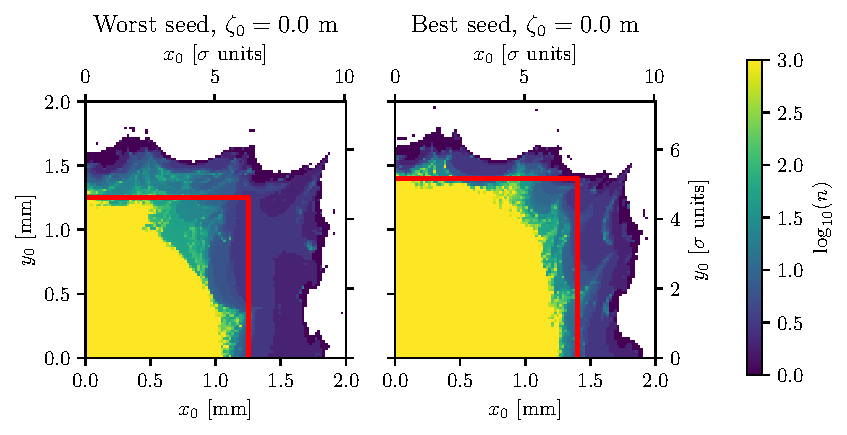
\includegraphics[width=0.8\textwidth]{6_lhc_dynamic_indicators/figs/quick_scan.pdf}
    \caption{Survival plot up to $n=10^3$ turns of two different seeds of a realistic HL--LHC lattice of Beam 1, without beam-beam interaction, at \SI{7.0}{TeV}. The two seeds achieved, the worst and best dynamic aperture value out of the selection of 60 seeds available. The initial conditions consist of a $100\times100$ grid over the $x-y$ transversal plane. A region of interest (ROI) is highlighted in red on the two survival plots, and represents the choice of boundaries for the finer sampling we performed for our dynamic indicator analysis.}
    \label{fig:seed_presentation}
\end{figure}

To inspect the performance of the dynamic indicators, we sampled initial conditions on a uniform Cartesian grid of $300\times300$ particles in the $x-y$ plane, with transverse moments $p_x$ and $p_y$ set to zero. The boundaries of the Cartesian grid were manually selected based on the scan results presented in Fig.~\ref{fig:seed_presentation}, to have a square region of interest (ROI) focused on the dynamic aperture region highlighted at $n=10^3$. The boundary of the selected ROI is coloured red.

The longitudinal variable $\zeta$ was set at three values to inspect different levels of tune modulations induced by synchrotron motion, respectively, at \SI{0.0}{\meter}, at \SI{0.15}{\meter}, which is halfway close to the bunch separatrix, and at \SI{0.3}{\meter}, which is very close to the bucket separatrix. See Fig.~\ref{fig:the_bunch} for an illustration of the chosen $\zeta$ values, which are based on the tracking results of multiple initial conditions with different initial $\zeta$ values and $x, p_x, y, p_y$ set to zero. 

\begin{figure}
    \centering
    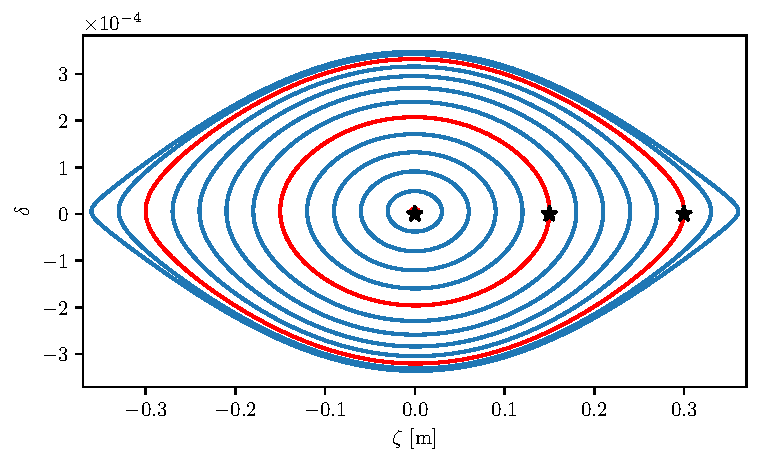
\includegraphics[width=0.65\textwidth]{6_lhc_dynamic_indicators/figs/longitudinal.pdf}
    \caption{Tracking of initial conditions with different $\zeta$ values up to $n=10^3$ on the HL-LHC lattice with best seed. The tracking highlights the classic structure, with the hyperbolic fixed points placed at $\zeta \sim \pm$ \SI{0.36}{\meter}. The three black crosses represents the three choices of $\zeta_0$ we decided to inspect in our dynamic indicator study.}
    \label{fig:the_bunch}
\end{figure}

\section{Chaos detection studies} \label{sec:8:results}

The dynamic indicators presented in the previous section, namely $FLI/n$, $FLI^{WB}$, $GALI^{(k)}$, $REM$, and $FMA$, were evaluated for the HL-LHC lattices up to $n=10^5$ turns. The results of the evaluation of these indicators are presented in the following sections.

Note how we present most of the value distributions on logarithmic scale, since the indicators are expected to follow either a power-law distribution or an exponential one. The logarithmic scale allows us to better inspect the tails of the distribution and the general tendencies of these indicators to create bimodal distributions, with the sole exception of $FMA$, which, as we have seen from the results in the previous chapter when considering a modulated Hénon map, tends to generate a trimodal distribution.

\subsection{Overview of the chaotic regions of the HL-LHC lattice}

The inspected $300\times300$ Cartesian grid of initial conditions considered in the selected ROIs gives us an overview of the phase space that ranges from zero amplitude to approximately 5 $\sigma$ units of amplitude.

An initial overview of how the phase space is structured is shown in Fig.~\ref{fig:true_survivors}, where we report a survival plot for the various configurations of the HL-LHC, in terms of the seed used and the value of $\zeta_0$ considered, tracked up to $n=10^5$ turns. As $n$ increases, a progressive erosion-like process takes place in the region where the particles are still not lost. This phenomenon is well known in the literature and has been studied for the development of dynamic aperture scaling laws, based on the Nekhoroshev theorem~\cite{Bazzani:2019csk}, which describes an exponentially slow decrease in dynamic aperture.

We can now inspect these six HL-LHC configurations with dynamic indicators and see what structures they highlight within the region where the particles survive up to $n=10^5$ turns. In Fig.~\ref{fig:fli_all}, we present a colour map of the values of $\log_{10}(\mathrm{FLI}(\hat{x})/n)$ evaluated in the six configurations. We can see, as expected, how chaotic regions, corresponding to the higher values of the indicator, occur at the borders of the stable region, showing for the case of certain configurations isolated structures that resemble islands of stability, with regular initial conditions within. These structures can be related to non-linear resonance effects. On the contrary, the internal core region is fully constituted by initial conditions with regular behaviour.

\begin{figure}
    \centering
    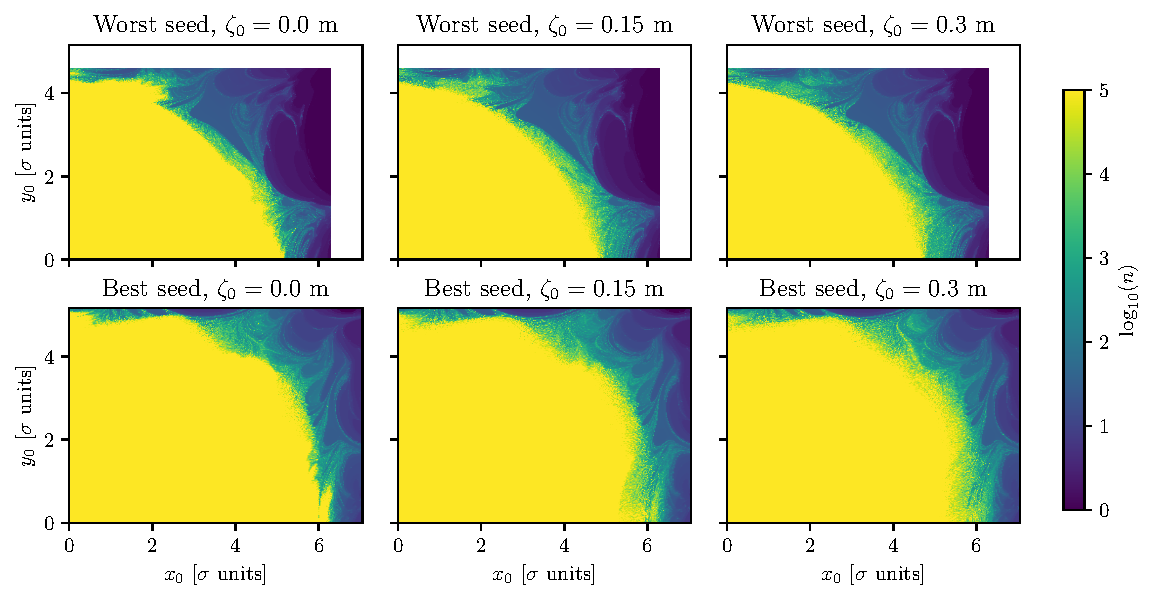
\includegraphics[width=0.9\textwidth]{6_lhc_dynamic_indicators/figs/stability.pdf}
    \caption{Survival plot up to $n=10^5$ turns for all six configurations of the realistic HL-LHC lattice model considered. The realization given by the seed causes strong changes in the phase space structure, while the initial value of $\zeta_0$ is related to different levels of erosion of the stable boundary.}
    \label{fig:true_survivors}
\end{figure}

\begin{figure}
    \centering
    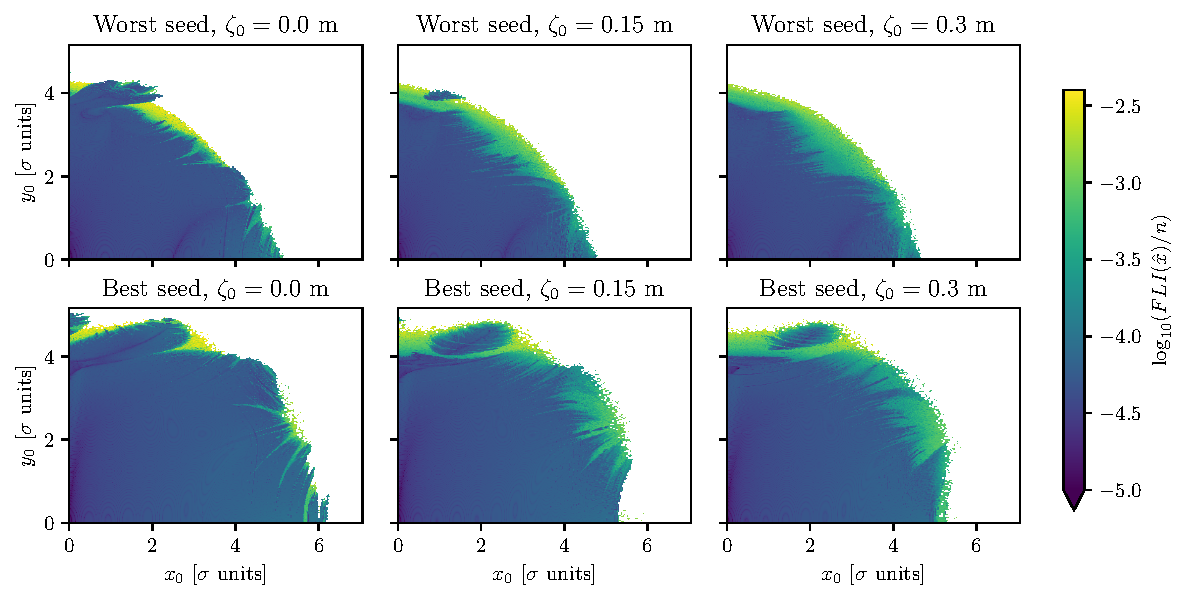
\includegraphics[width=0.9\textwidth]{6_lhc_dynamic_indicators/figs/fli_all.pdf}
    \caption{$\log_{10}(\mathrm{FLI}(\hat{x})/n)$ evaluated at $n=10^5$ for all six configurations of the realistic HL-LHC lattice model considered. The size of the chaotic structures highlighted by the indicator appears to be strongly correlated to $\zeta_0$.}
    \label{fig:fli_all}
\end{figure}

The size and shape of the chaotic regions appear to depend both on the seed and the initial value of $\zeta_0$. The worst seed also features larger regions of chaos in the phase space, while the best seed has the smallest among the three inspected. We can also see how increasing $\zeta_0$ contributes to slightly enlarging the size of chaotic regions, since the introduction of stronger longitudinal dynamics causes more modulation effects in the transverse plane, leading to more chaotic initial conditions. 

While we expect to see in the various lattices a correlation between the presence of large chaotic regions and a faster dynamic aperture decrease over time, we must stress that it is not a correct approach, nor the target of this paper, to seek a direct connection between the Lyapunov exponent of an initial condition and its stability time, as it is well known that there is no universal scale law connecting the two quantities, since such relation is extremely model dependent~\cite{Morbidelli1995}.

However, it is of interest to inspect the average value of the Lyapunov time (that is, the inverse of the maximum Lyapunov exponent~\cite{Tancredi_2001}) at different amplitudes. In Fig.~\ref{fig:ts_vs_r0}, we plot the inverse value of $FLI/n$, evaluated at $n=10^5$, with increasing amplitude. We can see how the values follow an exponential-like scale law. This functional shape resembles a Nekhoroshev-like scale law (i.e.\ Eq.~\eqref{nekest}), which found multiple applications in the definition of dynamic aperture scale laws.

In Fig.~\ref{fig:overview}, we present an overview of the various dynamic indicators in the analysis evaluated for one of the HL-LHC lattices, in the form of colour maps evaluated at $n=10^5$. We can see how the various dynamic indicators, with the exception of $FMA$, tend to highlight the same regions of chaos, giving a coherent overall evaluation of the phase-space chaoticity. The exception given by $FMA$ will be commented on in a later section. 

In Fig.~\ref{fig:overview2}, we present an overview of the evolution of the value distribution of the various dynamic indicators for different values of $n$. We can see that, in general, dynamic indicators tend to converge into a bimodal distribution, with the sole exception of $FMA$, which instead converges into a trimodal distribution. This tendency confirms what we observed in the previous chapter on the modulated Hénon map.

\begin{figure}
    \centering
    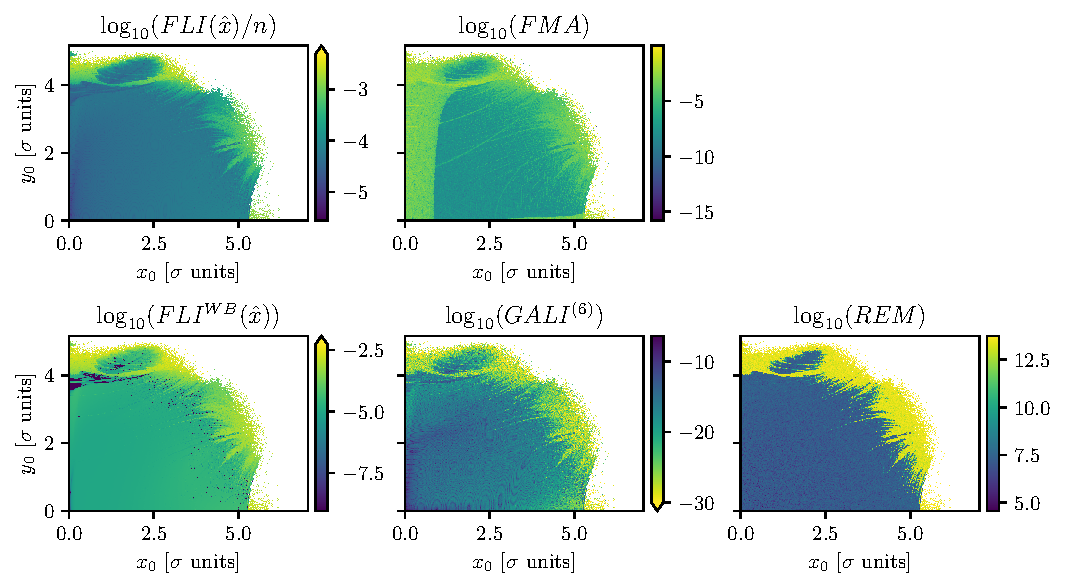
\includegraphics[width=1.0\textwidth]{6_lhc_dynamic_indicators/figs/overview.pdf}
    \caption{Colour maps of the various dynamic indicators for a realistic HL-LHC lattice, evaluated at $n=10^5$. It can be seen how the indicators globally highlight the same structures in phase space, with the exception of $FMA$, which also shows additional structures. (HL-LHC lattice used: best seed, $\zeta_0=$\SI{0.3}{\meter}.)}
    \label{fig:overview}
\end{figure}

\begin{figure}
    \centering
    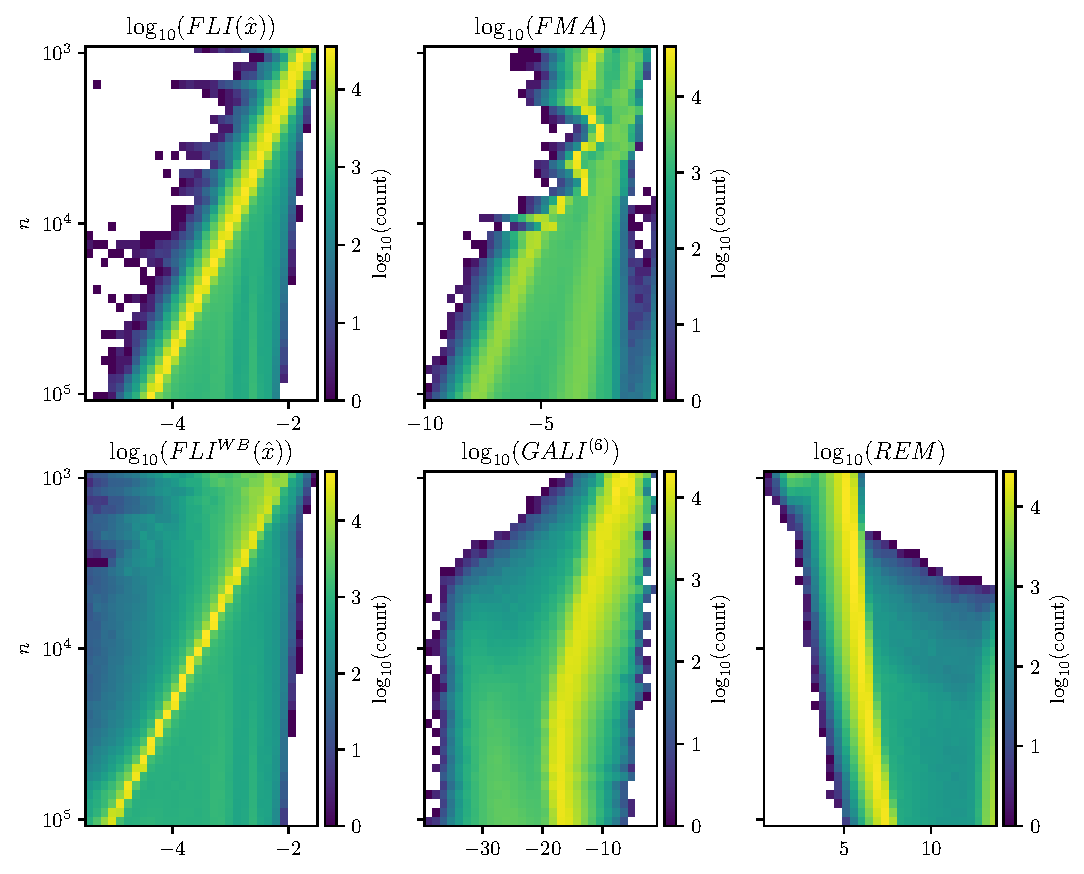
\includegraphics[width=1.0\textwidth]{6_lhc_dynamic_indicators/figs/evolution.pdf}
    \caption{Distribution of values of the various dynamic indicators as a function of time for a realistic HL-LHC lattice. For low values of the number of turns $n$, the distribution is in general represented by a uni-modal function. For higher values of $n$, we can see the formation of either two separate clusters, making the distribution bi-modal, or an individual cluster with a significant tail. $\log_{10}(FMA)$ constitutes an exception, as it evolves forming a tri-modal distribution. (HL-LHC lattice used: best seed, $\zeta_0=$\SI{0.3}{\meter}.)}
    \label{fig:overview2}
\end{figure}

\section{Some characteristics of dynamic indicators}\label{sec:8:features}

\subsection{$FLI$ dependence on the initial displacement}

$FLI$, by definition, depends on the initial choice of the direction of the unitary displacement vector $\vb{\xi}$, which implies that different structures can be highlighted in the phase space.

To assess the magnitude of these differences, in Fig.~\ref{fig:fli_compare}, we compare the calculated values of $\log_{10}({FLI})$, calculated at $n=10^5$ with an initial displacement along one of the six orthonormal vectors, namely $\hat{x},\,\hat{p}_x,\,\hat{y},\,\hat{p}_y,\,\hat{\zeta},\,\text{and }\hat{\delta}$. The comparison is made against the mean value computed for the six possible initial displacements and the standard deviation is also presented.

It is possible to see how the different choice of initial displacement highlights different structures in the regular region, whereas chaotic regions tend to assume the same final value. This difference is also highlighted by the standard deviation, since the chaotic regions at the border generally show a low standard deviation, whereas the stable regions at lower amplitude have higher values.

This result is to be expected, as chaotic initial conditions are characterized by a large maximal Lyapunov exponent, which leads different initial displacements to eventually align along it after a high enough number of turns. However, in contrast, regular initial conditions may not exhibit this preferential direction and lead to greater differences in $FLI$ values for different initial conditions. However, it is important to highlight the fact that the general character of the dynamic indicator stays consistent along the various directions and at most causes slight evaluation differences for the initial conditions close to the border between a regular and a chaotic region in the phase space.

\begin{figure*}[htp]
    \centering
    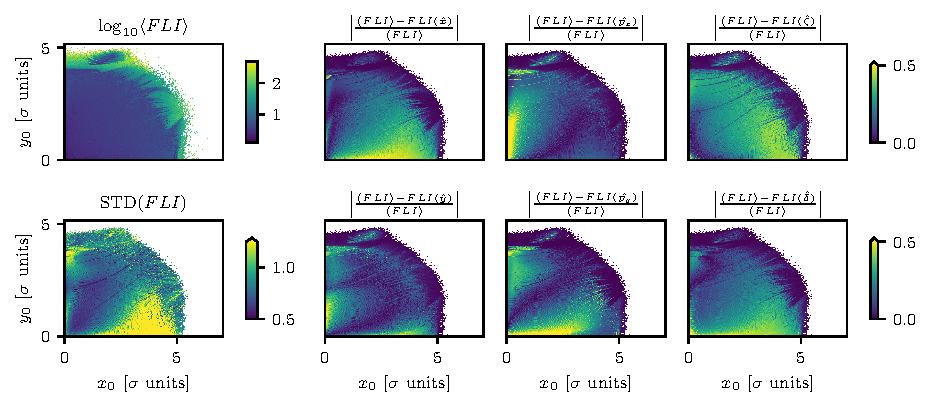
\includegraphics[width=1.0\textwidth]{6_lhc_dynamic_indicators/figs/LE_FLI_high_main_idx_8.pdf}
    \caption{Overview of $FLI$ evaluated at $n=10^5$ using as initial displacement any of the six base vectors $\hat{x},\,\hat{p}_x,\,\hat{y},\,\hat{p}_y,\,\hat{\zeta},\,\text{and }\hat{\delta}$. The two colour maps on the left show the mean and the standard deviation of all six evaluations of $FLI$, the others show the values of $FLI$ for each of the six initial displacements as relative difference from the mean value. (HL-LHC lattice used: best seed, $\zeta_0=$\SI{0.3}{\meter}.)}
    \label{fig:fli_compare}
\end{figure*}

\subsection{Use of Birkhoff weights with $FLI$}

To quantify the convergence improvements given by the Birkhoff weights, we compare the values obtained for $FLI$ at different times for one of the HL-LHC lattices, using either the standard approach that considers the mean in Eq.~\eqref{eq:fli_mean}, that is, $FLI/n$, or the weighted mean based on the use of Birkhoff weights as in Eq.~\eqref{eq:fli_birkhoff}, that is, $FLI^{WB}$.

In this analysis, we consider two ensembles of regular and chaotic particles that have been classified by means of the value of the $FLI$ indicator computed for $n=10^5$ turns. In this context, we consider regular particles those that have reached a final value of $\log_{10}(\mathrm{FLI}/n) < -4.5$, and, as chaotic particles, we consider those that have reached a final value of $\log_{10}(\mathrm{FLI}/n) > -2.5$. This arbitrarily thresholding is based on the expected properties of the dynamic indicator $FLI$ and considers a subset of initial conditions that have already manifested clear regular or chaotic behaviour at $10^5$ turns, while excluding those that do not yet have a clear classification.

The sets are then used to inspect the time evolution of both $FLI/n$ and $FLI^{WB}$, to assess possible classification improvements in the latter compared to the first. These improvements can be, for example, an increased convergence rate in the indicator value or an increased spread between the values of regular and chaotic initial conditions.

In Fig.~\ref{fig:fli_compare_mean_birk_2} (left), the comparison between the two indicators is made for a subset of the set of regular initial conditions. It is possible to observe how, for regular initial conditions, Birkhoff averaging does not seem to significantly improve the convergence rate, although it does introduce a constant shift towards a smaller indicator value gap that improves the overall performance of the indicator.

\begin{figure}[htp]
    \centering
    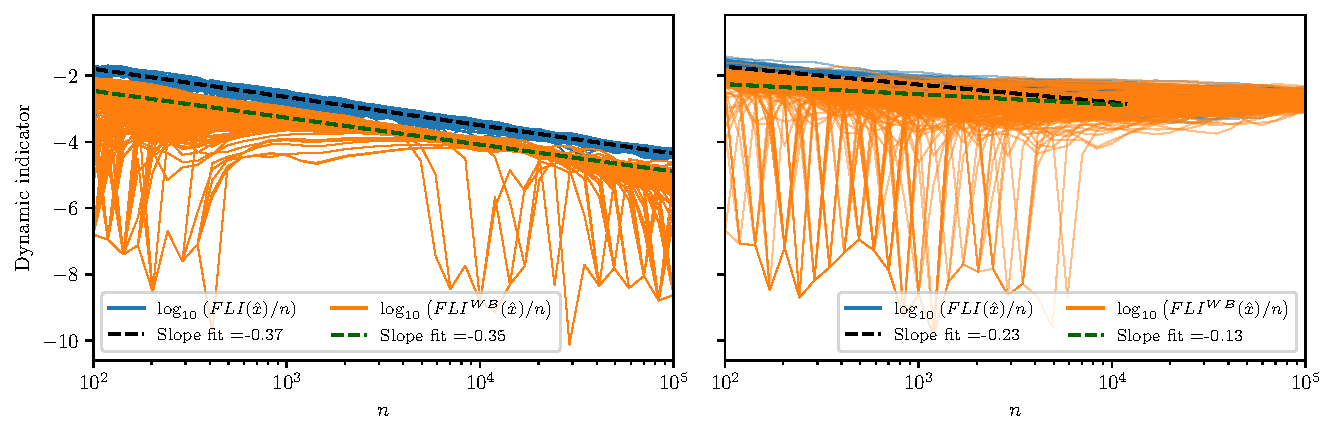
\includegraphics[width=1.0\textwidth]{6_lhc_dynamic_indicators/figs/fli_vs_flibk_idx_2.pdf}
    \caption{Time evolution of $FLI$ computed using either a standard mean ($FLI/n$) or the Birkhoff averaging ($FLI^{WB}$). Left plot: indicators computed for a set of $100$ regular initial conditions, the fit highlights an almost identical convergence rate for the two indicators, although the Borkhoff averaging introduces a constant shift towards a smaller indicator value, which represents already an improvement. Right plot: indicators computed for a set of $100$ chaotic initial conditions. A slight difference in convergence rate is observed for low $n$ values, before reaching a saturation value of the indicator of the order of $10^{-3}$. (HL-LHC lattice used: worst seed, $\zeta_0=$\SI{0.3}{\meter}.)}
    \label{fig:fli_compare_mean_birk_2}
\end{figure}

In Fig.~\ref{fig:fli_compare_mean_birk_2} (right), we show the comparison for the subset of chaotic initial conditions. In this case, a saturation region is observed for the indicator value of the order of $10^{-4}$ for both indicators. When this value is reached, both indicators oscillate around it. However, the slope with which this non-zero value is reached is different for the two indicators and is higher in absolute value for $FLI^{WB}$ than for $FLI/n$. We must also point out how some chaotic initial conditions exhibit large fluctuations in $FLI^{WB}$ before the saturation point, reaching values comparable to the regular initial conditions. These isolated cases might be artefacts caused by the Birkhoff weights, which amplify certain modes in the time series when the chaotic behaviour still has not fully manifested.

Despite these isolated oscillations, the improvement brought about by the Birkhoff averages can be appreciated by comparing the evolution of the value distribution of $\log_{10}(FLI/n)$ and $\log_{10}(FLI^{WB})$ reported in Fig.~\ref{fig:overview2}, since there the time evolution of the value distribution is shown for all the initial conditions shown in Fig.~\ref{fig:overview}. The part of the distribution corresponding to the regular initial conditions reaches its peak (yellow band) and moves toward zero with increasing $n$. However, the displacement toward zero is faster for $FLI^{WB}$, and the peak is also narrower, potentially allowing for a better classification method, as seen in the previous chapter. It should be stressed that, as already mentioned, the lower values of $FLI^{WB}$ are not due to a steeper slope, but to a constant initial offset. In both graphs, a faint trace of a peak is visible that corresponds to the indicator value of about $10^{-3}$. This feature is remarkably similar for the two indicators, as already seen in Fig.~\ref{fig:fli_colormap_mean_birk}.

When applied to a modulated Hénon map, as discussed in Section~\ref{subsec:dyn:FLI:WB}, the Birkhoff weights applied to $FLI$ provided a slight improvement in the convergence of regular initial conditions to zero, as well as an overall benefit in highlighting the two separate clusters of initial conditions. In the current context, this difference in convergence was not appreciated to a comparable extent; however, a slight improvement was observed in cluster sharpness and separation, suggesting that Birkhoff weights still offer a certain improvement with respect to the plain $FLI$ classification of chaotic orbits. 

\subsection{Dependence of $FMA$ from the longitudinal dynamics}

As observed in Appendix~\ref{app:timedep}, the chaotic structures highlighted by $FMA$ are very different from those highlighted by the other dynamic indicators. This is due to the fact that $FMA$ is generally sensitive to tune changes, which are not necessarily related to chaotic dynamics, but rather related to the presence of resonances or tune modulation.

To further highlight this characteristic of $FMA$, we can observe how the indicator is particularly sensitive to the presence of longitudinal dynamics. Indeed, the longitudinal dynamics couples with the transverse one, also introducing tune modulation via a finite value of the chromaticity. In Fig.~\ref{fig:fma_vs_fli}, we present $FMA$ evaluated for the best seed for three values of $\zeta_0$, and we compare the resulting structures with those highlighted by $FLI^{WB}$. Two essential features can be observed. The first is that the chaotic regions at the border of the stable region resemble very much for the two indicators, which show that their behaviour is similar. The second is a strong difference between the two indicators in the region close to the vertical axis. This difference grows significantly as a function of $\zeta_0$. 
%
\begin{figure}[ht]
    \centering
    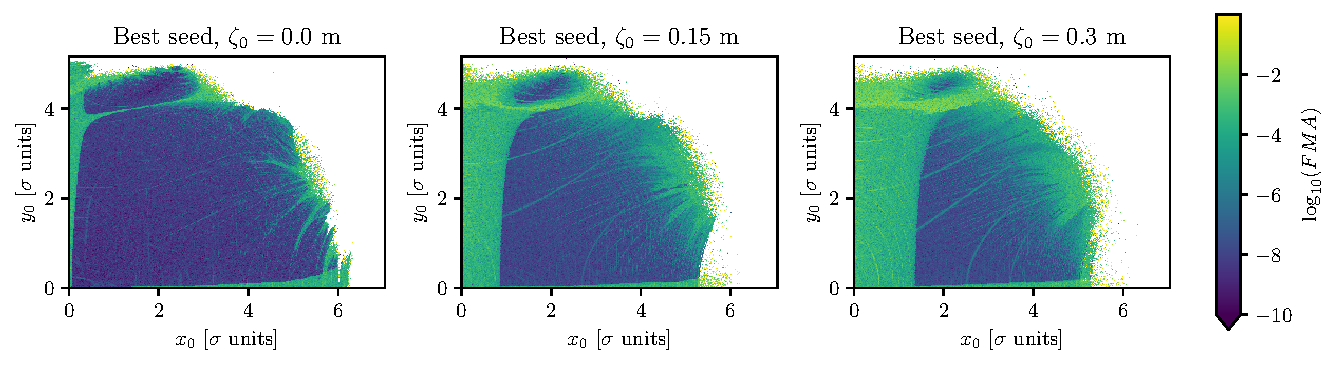
\includegraphics[width=1.0\textwidth]{6_lhc_dynamic_indicators/figs/FMA.pdf}
    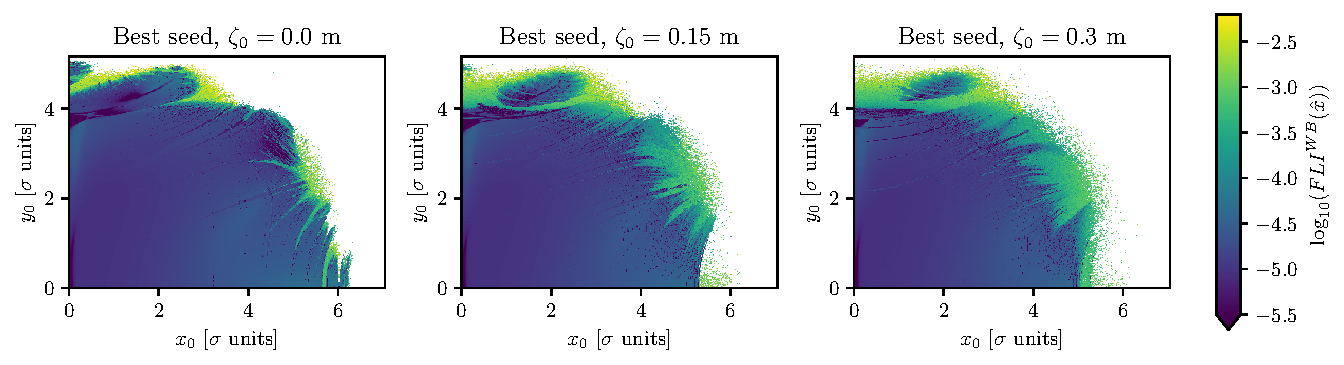
\includegraphics[width=1.0\textwidth]{6_lhc_dynamic_indicators/figs/FMA_addendum.pdf}
    \caption{$\log_{10}(\mathrm{FMA})$ (top row) and $\log_{10}(\mathrm{FLI}^{WB}(\hat{x}))$ (bottom row) evaluated on the same seed for three values of $\zeta_0$ at $n=10^5$. The differences between the two indicators are enhanced with larger values of $\zeta_0$.}
    \label{fig:fma_vs_fli}
\end{figure}
%
With increasing values of $\zeta_0$ the chaotic region detected by $FMA$ extends toward the origin along the vertical axis. Furthermore, the width of this chaotic region increases with $\zeta_0$. It is quite clear that the chaotic behaviour detected by $FMA$ is an artefact related to the presence of a strong modulation of the tunes. In this sense, this observation suggests that the use of $FMA$ to identify chaotic regions in phase space is taken with a grain of salt whenever modulation of linear tunes is present.   

Another feature emerges when considering the evolution of the distribution of indicator values as a function of time. In fact, if we compare the evolution of the value distribution of $FMA$, we can observe how $FMA$ evolves into a trimodal distribution. Unlike the other dynamic indicators, which show a tendency to create a bimodal distribution.

\subsection{General performance of $REM$}

In the previous chapter, the performance of different dynamic indicators was evaluated using a modulated Hénon map and applying a clustering approach to detect chaotic orbits. This analysis showed that the $REM$ indicator is capable of highlighting chaotic structures faster than Lyapunov-based dynamic indicators such as $FLI^{WB}$. Mainly because of its ability to distinguish regular orbits from chaotic ones in a well-defined bimodal distribution, as the numerical error is quickly amplified by the chaotic character of the orbits.

When applying $REM$ to the HL-LHC lattices, we observe a similar behaviour, i.e.\ the ability to clearly highlight chaotic regions in the phase space. In Fig.~\ref{fig:overview}, we can qualitatively compare the results obtained by $REM$, calculated for an example seed, with those obtained with $FLI^{WB}$. We can observe how $REM$ tends to highlight chaotic regions qualitatively sharper than $FLI^{WB}$, reproducing the same behaviour observed in the modulated Hénon map, although, for this analysis, we lack the possibility to define a ground truth to be used to compare the results of the various indicators.

The behaviour of the distribution of the indicator values can be appreciated by comparing the evolution of the value distribution of $\log_{10}(REM)$ and $\log_{10}(FLI^{WB})$ as a function of time, as shown in Fig.~\ref{fig:overview2}. In fact, $\log_{10}(REM)$ tends to a bimodal distribution much faster than $\log_{10}(FLI^{WB})$ and in such a way that a threshold for detecting chaotic initial conditions would be almost independent of $n$. Therefore, we can conclude that the promising performance of $REM$ in highlighting chaotic structures in the phase space, along with its straightforward numerical implementation, makes it a very interesting tool for studying phase-space structures in realistic accelerator lattices.

\section{Analysis of the beam dynamics using dynamic indicators}\label{sec:8:detailed}

\subsection{Considerations on stability time and Lyapunov time}

The Lyapunov time $T_\mathrm{L}$ is defined as the inverse of the maximal Lyapunov exponent of the system, which is directly estimated by the dynamic indicators $FLI/n$ and $FLI^{{WB}}$.

We are interested in assessing whether $T_\mathrm{L}$ follows a Nekhoroshev-like scaling law, which would indicate that the chaotic regions are those contributing to the diffusion-like process that has been introduced in the proposed framework. In other words, we want to inspect whether $T_\mathrm{L}$ scales with the amplitude $I$ of an initial condition, such as in Eq.~\eqref{nekest}. This study is motivated by the well-known fact that the dynamic aperture follows a Nekhoroshev-like evolution~\cite{Bazzani:2019csk}, discussed in Section~\ref{sec:2:dynamic_aperture}, which implies a scaling law that describes an exponential reduction in the stability time $T_\mathrm{s}$ of the initial conditions as a function of their initial amplitude $I_0$.

To make use of our numerical simulation data and inspect $T_\mathrm{s}$ and $T_\mathrm{s}$ as functions of the initial radius $r_0 = \sqrt{x_0^2 + y_0^2}$ of an initial condition, we evaluated the mean values of $T_\mathrm{s}$ and $T_\mathrm{L}$ for a set of initial conditions in the amplitude interval $]r_0-\Delta r/2, r_0 +\Delta r/2[$. The mean values of $T_\mathrm{s}$ and $T_\mathrm{L}$ are then calculated for each interval and the resulting values are plotted as a function of $r_0$. Note that for our Nekhoroshev-like scaling laws, $I_0$ and $r_0$ are related by $I_0 = r_0^2$.

To evaluate an optimal choice for $\Delta r$, we first calculate the mean values of $T_\mathrm{s}$ and $T_\mathrm{L}$ for a range of values of $\Delta r$, and compare the resulting curves directly. We then select the value of $\Delta r$ as the best compromise between statistical fluctuations and loss of information. In Fig.~\ref{fig:ts_vs_r0}, we present the results of this analysis for both $T_\mathrm{s}$ and $T_\mathrm{L}$, applied to one of the realisations of the HL-LHC lattice. We can observe that the best compromise is achieved for $\Delta r = 0.2\sigma$, which is the value used in the following.

\begin{figure}
    \centering
    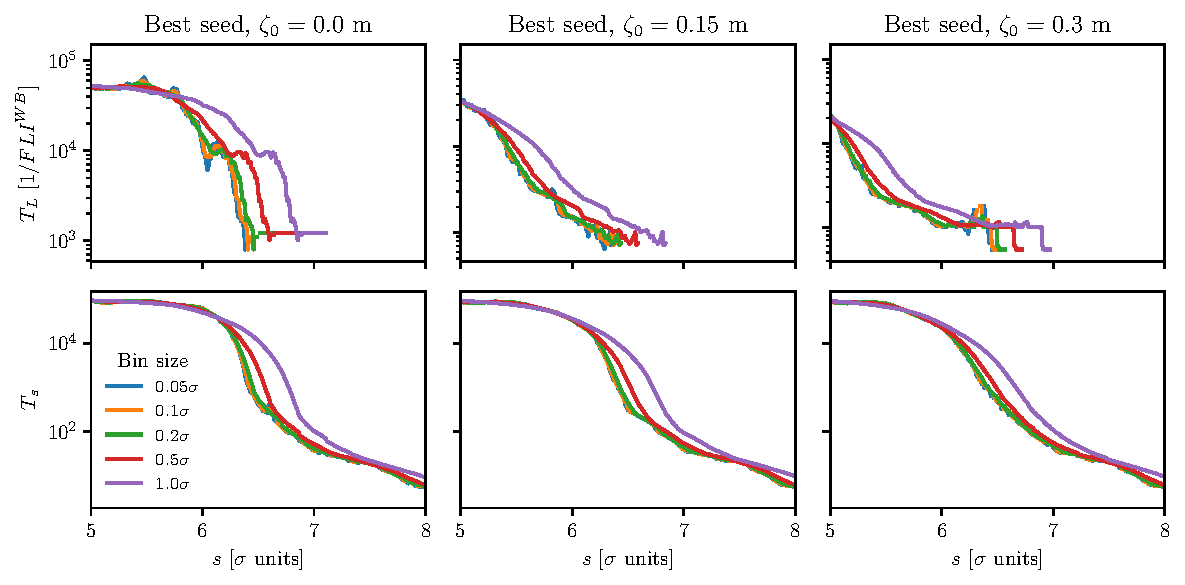
\includegraphics[width=1\textwidth]{6_lhc_dynamic_indicators/figs/lyapunov_time_vs_thickness.pdf}
    \caption{Mean values of $T_\mathrm{s}$ and $T_\mathrm{L}$ as a function of $r_0$ for some values of $\Delta r$. The best compromise between statistical fluctuations and loss of information is achieved for $\Delta r = 0.2\sigma$.}
    \label{fig:ts_vs_r0}
\end{figure}

To estimate the Lyapunov time $T_\mathrm{L}$, we can use $FLI/n$ or $FLI^{{WB}}$, as they both provide an estimate of the maximal Lyapunov exponent and hence of $T_\mathrm{L}$. In Fig.~\ref{fig:lyapunov_time_fli_vs_wb}, we present the results of this analysis for the same seed of the HL-LHC lattice. For regular orbits, the maximal Lyapunov exponent is zero, and therefore $T_\mathrm{L}$ is infinite. For chaotic orbits, however, the maximal Lyapunov exponent is finite, and therefore $T_\mathrm{L}$ is finite as well. However, since the $FLI/n$ and $FLI^{WB}$ dynamic indicators are evaluated at a finite time $n$, it is inevitable to observe a non-zero value of the maximal Lyapunov exponent, and hence a finite value of $T_\mathrm{L}$, also for regular orbits. This can be observed in Fig.~\ref{fig:lyapunov_time_fli_vs_wb}, since for values of $r_0$ corresponding to the regular regions of the phase space, i.e. close to zero, $T_\mathrm{L}$ as computed using $FLI/n$ tends to $10^5$, the maximum number of turns used in the numerical simulations. The situation is different for the case of $FLI^{{WB}}$. In fact, thanks to its superconvergence properties, it provides the same mean $T_\mathrm{L}$ value as $FLI/n$ for $r_0$ in the chaotic regions, i.e. corresponding to large values of $r_0$. Moreover, it provides higher values of $T_\mathrm{L}$ for $r_0$ corresponding to regular regions. 
On the basis of this observation, we will use $FLI^{{WB}}$ to derive $T_\mathrm{L}$ in the following.

\begin{figure}
    \centering
    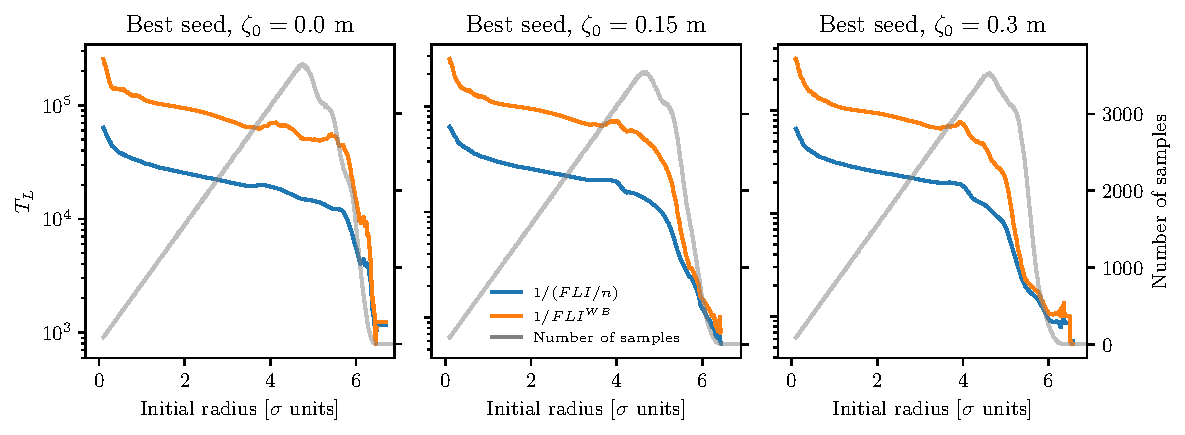
\includegraphics[width=1\textwidth]{6_lhc_dynamic_indicators/figs/lyapunov_time_vs_lyapunov_wb_time.pdf}
    \caption{Mean values of $T_\mathrm{L}$ as a function of $r_0$ with $\Delta r = 0.2\sigma$ for three values of the $\zeta_0$ variable. The results presented refer to $FLI/n$ and $FLI^{{WB}}$, both evaluated at $n=10^5$. For high values of $r_0$, the two indicators provide similar results, while for low values of $r_0$, $FLI^{{WB}}$ provides a higher value of $T_\mathrm{L}$. This is linked to the faster convergence rate of $FLI^{{WB}}$ to the true value of the indicator, and hence of the maximal Lyapunov exponent. The grey line represents ??.}
    \label{fig:lyapunov_time_fli_vs_wb}
\end{figure}

When comparing directly $T_\mathrm{L}$ and $T_\mathrm{s}$, as shown in Fig.~\ref{fig:ts_vs_tl}, we can observe that the two times exhibit a similar behaviour with respect to $r_0$: they both exhibit a saturated plateau for low $r_0$, corresponding to the region dominated by regular orbits, and an exponential decay beyond a certain values of the radius, which varies in sharpness and position depending on the value of $\zeta_0$. In the same figure, we also show different evaluations of $T_\mathrm{L}$ based on $FLI^{WB}$, evaluated at different values of $n$, which clearly show how the value of $T_\mathrm{L}$ for regular orbits increases with the value of $n$, while the value of $T_\mathrm{L}$ for chaotic orbits converges to its true value. Another important feature is clearly seen in the same figure, namely that $T_\mathrm{L}$ extends over a reduced range of $r_0$ values. This is due to the choice that the indicator values have been evaluated only for orbits that are stable up to $10^5$ turns, which explains clearly why, on the other hand, $T_\mathrm{s}$ extends over a wider range of $r_0$ values. 

The curves shown so far are obtained by a process of averaging of the raw data. To better appreciate the situation, the distributions of $T_\mathrm{L}$ and $T_\mathrm{s}$ as a function of $r_0$ are shown in Fig.~\ref{fig:extra_distribution}. There, the distributions are represented using a colour map and the mean values are highlited by the red curves. We can observe how the distributions feature a spread that correlates with the value of $r_0$, i.e. it shrinks towards small values of $r_0$ and grows with increasing values of $r_0$. For the case of $T_\mathrm{s}$, this effect is really striking as for $r_0$ values corresponding to the stable region of phase space the distribution of $T_\mathrm{s}$ is delta-like centred on the value of $10^5$. Indeed, the behaviour of the width of the distributions is not a surprising feature, as the value of $r_0$ is somewhat correlated with the presence of regular or chaotic orbits. 

\begin{figure}
    \centering
    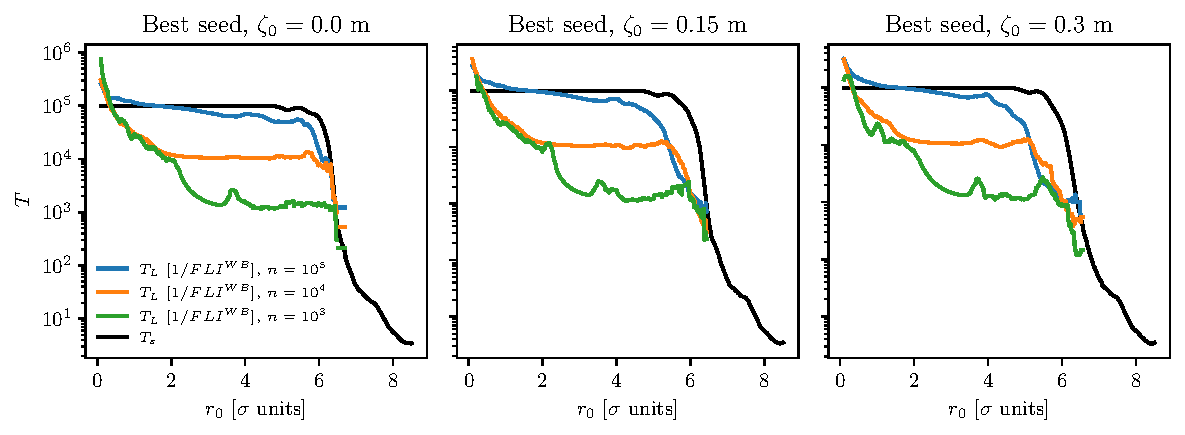
\includegraphics[width=1\textwidth]{6_lhc_dynamic_indicators/figs/lyapunov_time_vs_radius.pdf}
    \caption{Mean values of $T_\mathrm{L}$ and $T_\mathrm{s}$ as a function of $r_0$ for $\Delta r = 0.2\sigma$. The values of $T_\mathrm{L}$ are evaluated using $FLI^{{WB}}$ evaluated for three values of $n$. The convergence process of the reconstructed $T_\mathrm{L}$ is clearly visible. Differences and similarities of $T_\mathrm{L}$ and $T_\mathrm{s}$ are clearly visible. Also visible is the worsening of similarities between $T_\mathrm{s}$ and $T_\mathrm{L}$ for increasing values of the $\zeta_0$ variable. }
    \label{fig:ts_vs_tl}
\end{figure}

\begin{figure}
    \centering
    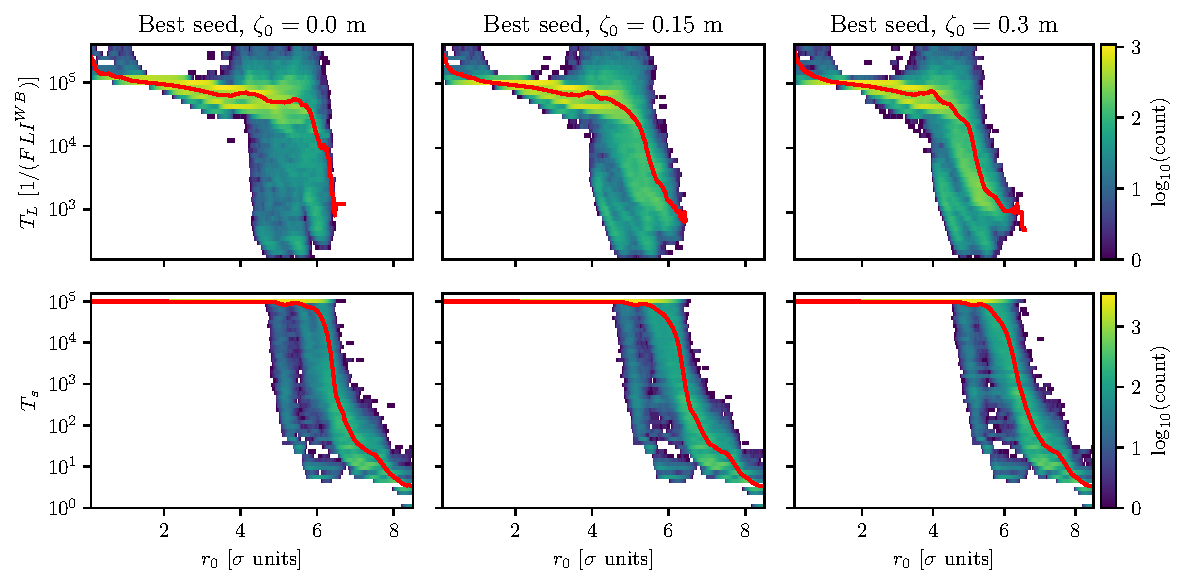
\includegraphics[width=1\textwidth]{6_lhc_dynamic_indicators/figs/dist_and_mean.pdf}
    \caption{Distribution of values of $T_\mathrm{L}$ (top) and $T_\mathrm{s}$ (bottom) as a function of $r_0$ for $\Delta r = 0.2\sigma$. The red lines represent the mean value of the distributions, which correspond to the black or blue lines of Fig.~\ref{fig:ts_vs_tl}.}
    \label{fig:extra_distribution}
\end{figure}

It is worth noting that given the shape of the distributions, the mean value does not correspond to the most probable one, i.e. the position of the maximum of the distribution. Therefore, we have evaluated the curves representing the most probable values of $T_\mathrm{s}$ and $T_\mathrm{L}$ and used for the following analyses. However, it turned out that the results of the fit discussed in the following are much less stable and because of this observation, the use of the most probable value of the distributions of $T_\mathrm{s}$ or $T_\mathrm{L}$ has been abandoned and the use of the mean value retained for the rest of the analyses.   

We now want to study the possibility of fitting a Nekhoroshev-like function
\begin{equation}
    T = T_0 \exp\left[-\left(\frac{I_\ast}{I_0}\right)^{\frac{1}{2\kappa}}\right]
\end{equation} 
to both $T_\mathrm{L}$ and $T_\mathrm{s}$, and analyse both the fit goodness and the dependence of the values of $T_0$, $I_\ast$, and $\kappa$ for the various combinations of realisations and values of $\zeta_0$. As this scale law ranges over multiple orders of magnitude, we consider the logarithm of $T$, and fit the following function:
\begin{equation}
    \log(T) = \log(T_0) - \left(\frac{I_\ast}{I_0}\right)^{\frac{1}{2\kappa}} \,.
\end{equation}

We first perform an initial brute-force search on a grid of values of $T_0$, $I_0^*$, and $1/(2\kappa)$, and then we carry out a more refined search around the best values found in the first step using the least squares method. The initial coarse-grained search is motivated by the non-linear nature of the fit, which makes it difficult to find the best values of the parameters with a simple gradient-descent method.

As we have seen in Figs.~\ref{fig:ts_vs_tl} and~\ref{fig:extra_distribution}, and as we discussed previously, the evaluation of $T_\mathrm{L}$ and $T_\mathrm{s}$ are inevitably affected by the nature of numerical simulations that are carried out over a finite number of turns, in our case $n=10^5$. Because of this, when performing the fit, we have to consider only the fraction of the data that does not show any saturation, which is determined by the finite number of turns used in numerical simulations. 

To make an accurate selection of the numerical data to be used for the fit, we perform the fit on various data sets, selected near the region of transition between the regular and chaotic regimes. We then choose the data cut that provides the best fit, using as a figure of merit the reduced $\chi^2$ of the fit.

Figure~\ref{fig:the_lyap_fit}, shows the result of the fitting procedure of $T_\mathrm{L}$ and $T_\mathrm{s}$, applied to two HL-LHC realisations, both with $\zeta_0=$ \SI{0.3}{\meter}. We can see how different choices of data selections lead to differences in the values of the fit parameters, and the optimal choice and data selection, and hence of fit parameters, can be made considering the reduced value $\chi^2$ which is also shown. 

\begin{figure}[htb]
    \centering
    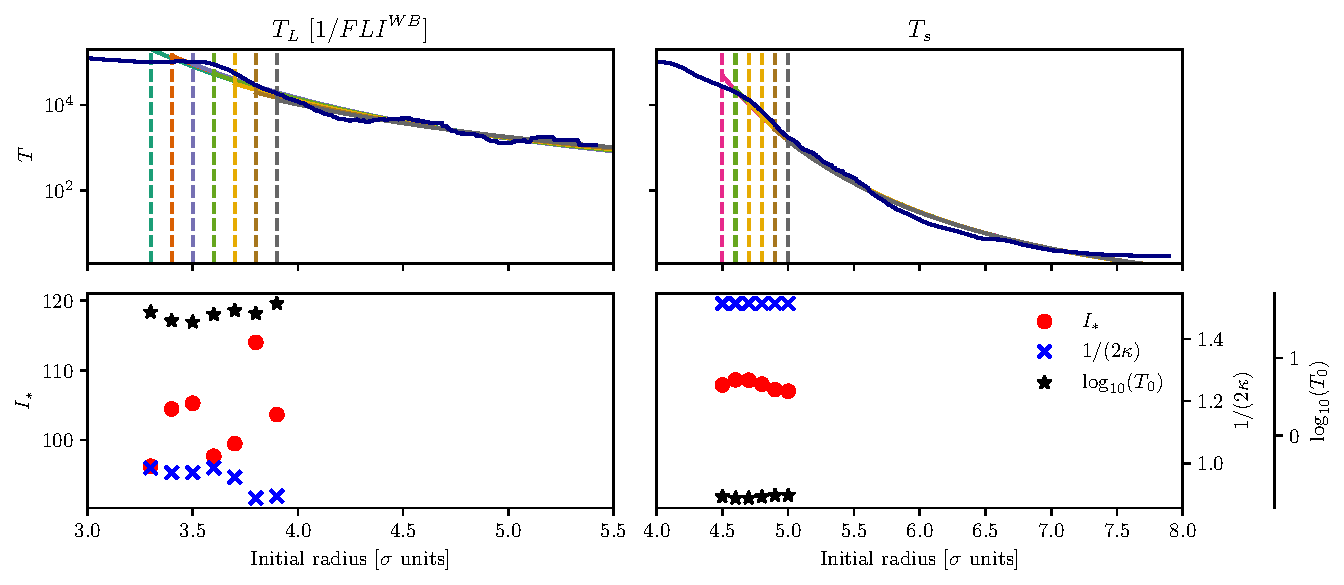
\includegraphics[width=1\textwidth]{6_lhc_dynamic_indicators/figs/fit_l_time_bad.pdf}
    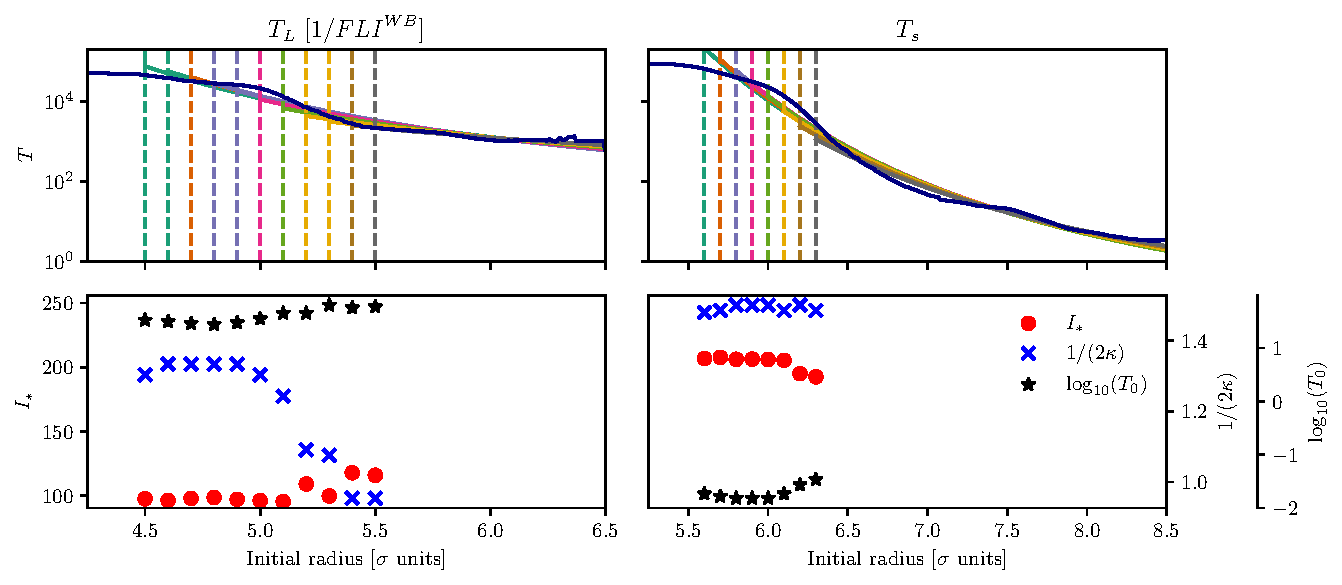
\includegraphics[width=1\textwidth]{6_lhc_dynamic_indicators/figs/fit_l_time_best.pdf}
    \caption{Results of the fit of $T_\mathrm{L}$ and $T_\mathrm{s}$ for two different HL-LHC realisations (top row, worst seed with $\zeta_0=$ \SI{0.3}{\meter}; bottom row, best seed with $\zeta_0=$ \SI{0.3}{\meter}). Multiple slices of data are considered close to the transition point at which the data begins to manifest clear saturation due to the finite tracking time. The best fit is chosen by considering the minimum of the reduced $\chi^2$ for the various data cuts considered. The values of the fit parameters are also shown.}
    \label{fig:the_lyap_fit}
\end{figure}

In Table~\ref{tab:lyap_fit_results}, we report the fit parameters obtained for the six combinations of HL-LHC configurations we have considered. We can observe how in general the fit routine archives reasonable error estimates for all the datasets, with the exception of the fitting of $T_\mathrm{L}$ for the initial conditions with $\delta_0 =$ \SI{0.0}{\metre}, where the small size of chaotic regions, due to the absence of strong chaotic contribution from the longitudinal-induced modulation, makes the fit routine unable to identify a valid Nekhoroshev-like scale law.

We can also observe how, in the $T_\mathrm{s}$ fit, all the exponents $1/(2\kappa)$ have comparable value. This is promising as $\kappa$ is a parameter that is related to the geometry of the phase space, and thus it is expected to be a constant for all the different seeds. Similarly, $I_\ast$ shows a coherent behaviour, as it appears strongly correlated to the seed choice and the value of $\zeta_0$, decreasing as the combination of the two creates a situation with less stability.

As for the $T_\mathrm{L}$ fit, other than the case of the initial conditions with $\delta_0 =$ \SI{0.0}{\metre}, we can observe how the values of $1/(2\kappa)$ are comparable only within the same seed, with the best seed being the one closest to the value achieved for the $T_\mathrm{s}$ fit. This suggests that the evolution of $T_\mathrm{L}$ follows a different geometry than the one of $T_\mathrm{s}$, and, as we will see shortly, this can be related to similar results in literature. 

\begin{table}[htb]
    \centering
    \begin{tabular}{l|c|ccc}
        \toprule
        \multicolumn{2}{c|}{$T_\mathrm{s}$ fit} & $\zeta_0=$ \SI{0.0}{\meter} & $\zeta_0=$ \SI{0.15}{\meter} & $\zeta_0=$ \SI{0.3}{\meter} \\
        \midrule
        \multirow{3}{*}{\makecell{Worst\\seed}}  & $1/(2\kappa)$ & $2.94 \pm 0.02$ & $3.0 \pm 0.2$ & $3.03 \pm 0.08$ \\
        & $I_\ast$ & $131 \pm 2$ & $119 \pm 7$ & $109 \pm 5$ \\
        & $\log_{10}(T_0)$ & $-1.23 \pm 0.04$ & $-0.95 \pm 0.08$ & $-0.81 \pm 0.06$ \\
        \midrule

        \multirow{3}{*}{\makecell{Best\\seed}}  & $1/(2\kappa)$ & $2.9997 \pm 0.0004$ & $3.03 \pm 0.07$ & $3.00 \pm 0.08$ \\
        & $I_\ast$ & $220 \pm 40$ & $208 \pm 28$ & $206 \pm 23$ \\
        & $\log_{10}(T_0)$ & $-2.2 \pm 0.3$ & $-1.9 \pm 0.3$ & $-1.819 \pm 0.004$ \\
        \bottomrule
    
        \toprule
        \multicolumn{2}{c|}{$T_\mathrm{L}$ fit} & $\zeta_0=$ \SI{0.0}{\meter} & $\zeta_0=$ \SI{0.15}{\meter} & $\zeta_0=$ \SI{0.3}{\meter} \\
        \midrule
        \multirow{3}{*}{\makecell{Worst\\seed}}  & $1/(2\kappa)$ & $1 \pm 3$ & $1.88 \pm 0.01$ & $1.9 \pm 0.1$ \\
        & $I_\ast$ & $2500 \pm 1600$ & $100 \pm 40$ & $104 \pm 31$ \\
        & $\log_{10}(T_0)$ & $-3 \pm 17$ & $1.9 \pm 0.3$ & $1.5 \pm 0.3$ \\

        \midrule
        \multirow{3}{*}{\makecell{Best\\seed}}  & $1/(2\kappa)$ & $1.5 \pm 1.0$ & $2.94 \pm 0.08$ & $2.7 \pm 0.1$ \\
        & $I_\ast$ & $1700 \pm 400$ & $108 \pm 25$ & $98 \pm 27$ \\
        & $\log_{10}(T_0)$ & $-4 \pm 5$ & $1.1 \pm 0.3$ & $1.5 \pm 0.3$ \\
        \bottomrule
    \end{tabular}

    \caption{Results of the fit of a Nekhoroshev-like scaling law on $T_\mathrm{s}$ and $T_\mathrm{L}$ data obtained from the six combinations of HL-LHC realisations and $\zeta_0$ values considered. The error reported is that associated to the fit procedure and represents the standard deviation of the fit parameters evaluated by the least-squares method.}
    \label{tab:lyap_fit_results}
\end{table}

In the work of Morbidelli et al.~\cite{Morbidelli1995}, an overview on the relationship between the Lyapunov time $T_\mathrm{L}$ and macroscopic instability times, which can be related to our measure of stability time $T_\mathrm{s}$, is presented. In particular, the authors distinguish between two different regimes, depending on the characteristics of the Hamiltonian dynamical system under study and the eventual presence of low-order resonances overlapping together.

The first regime is called the \textit{``resonance overlapping regime''}, and it is characterized by the presence of low-order resonances overlapping together. In this case, $T_\mathrm{s}$ is expected to be in a polynomial relation with $T_\mathrm{L}$, i.e.\ $T_\mathrm{s} \sim T_\mathrm{L}^\beta$, with some positive $\beta$. The second regime is called the \textit{``Nekhoroshev regime''}, and it is shown by the authors how such a regime can not follow a universal polynomial relation between $T_\mathrm{s}$ and $T_\mathrm{L}$, but might follow, instead, an exponential one, i.e.\ $T_\mathrm{s} \sim \exp(T_\mathrm{L})$. This highlights the fact that there is not a universal regime between $T_\mathrm{s}$ and $T_\mathrm{L}$, but rather a regime that depends on the specific characteristics of the Hamiltonian dynamical system under study.

If we bring forward our thesis that both $T_\mathrm{s}$ and $T_\mathrm{L}$ follow a Nekhoroshev-like scale law with respect to $I_0$, we can construct the following relation between the two values:
\begin{equation}
    \frac{T_\mathrm{s}}{T_{0s}} = \exp\left[\left(\frac{I_{\ast s}}{I_{\ast L}}\right)^{1/2\kappa_s}\left(\log\frac{T_\mathrm{L}}{T_{0L}}\right)^{\kappa_L / \kappa_s}\right] \, ,
\end{equation}
where, if $\kappa_L/\kappa_s = 1$, we are able to recover a polynomial relation between $T_\mathrm{s}$ and $T_\mathrm{L}$ in the form $T_\mathrm{s} = \alpha T_\mathrm{L}^\beta$. If this is not the case, the relation assumes the form $T_\mathrm{s} = \alpha \exp(\beta' \log{T_\mathrm{L}}^{\kappa_L / \kappa_s})$.

\subsection{Time evolution of $GALI^{(k)}$ for chaotic orbits}

The $GALI^{(k)}$ indicators depend on the value of the parameter $k$ that assumes the values $2 \leq k \leq 2N$, where $N$ is the number of degrees of freedom of the system, which, in our case, is $N=3$. For $k=6$ we have that the choice for the linearly independent initial displacements is rather obvious and corresponds to the six base vectors $\hat{x}$, $\hat{y}$, $\hat{p}_x$, $\hat{p}_y$, $\hat{\zeta}$, and $\hat{\delta}$, and a single indicator exists. On the other hand, for lower values of $k$, we can select the subspace of initial displacements among several possibilities and explore the chaotic behaviour of the system in that specific subspace.

The choice of $k$ has consequences on the convergence rate of the indicator for regular and chaotic orbits. A complete overview of the different expected behaviours of $GALI^{(k)}$ for different values of $k$ is given in~\cite{SKOKOS200730}.

If the orbit is chaotic, $GALI^{(k)}$ converges to zero exponentially fast with the law
\begin{equation}
    GALI^{(k)} \propto \exp\left[-t\left((\lambda_1 - \lambda_2)+(\lambda_1 - \lambda_3)+\cdots+(\lambda_1 - \lambda_k)\right)\right] \,,
\end{equation}
where $\lambda_1$ is the largest Lyapunov exponent and $\lambda_2> \lambda_3>\cdots>\lambda_k$ are the next $k-1$ Lyapunov exponents in decreasing order. If we assume $\lambda_1 \gg \lambda_2$, we see that the exponential decay of $GALI^{(k)}$ is bounded by $\exp(-tk\lambda_1)$.

In contrast, if the orbit is regular, $GALI^{(k)}$ varies with time according to different laws depending on the value of $k$ and the choice of displacements. That is, we have
\begin{equation}
    GALI^{(k)} \propto \begin{cases}\text { constant } & \text { if } 2 \leq k \leq N \\ \frac{1}{t^{2(k-N)-m}} & \text { if } N<k \leq 2 N \text { and } 0 \leq m<k-N \\ \frac{1}{t^{k-N}} & \text { if } N<k \leq 2 N \text { and } m \geq k-N\end{cases} \,.
\end{equation}

Therefore, in our case for $k\leq3$, the indicator should show a constant value over time, while for $k>3$ the indicator can show different power laws, depending on the value of $m$, which represents the dimensionality of the tangent space of the invariant torus on which the dynamics takes place.

These properties of the $GALI^{(k)}$ indicator make it a very useful tool for inspecting the geometrical properties of regular orbits in phase space. More specifically, studying the behaviour of $GALI^{(4)}$ for the various combinations of displacement vectors can give us an idea of the structure, i.e. dimensionality, of the regular orbits, by looking at the value assumed by $m$ assumes.

As a first attempt to test this behaviour with our HL-LHC lattices, we have inspected the evolution of the mean value of $GALI^{(2)}$ and $GALI^{(4)}$ for a set of regular initial conditions, selected using the indicator $FLI^{WB}$ calculated for $n=10^5$ turns. As displacement choices, we tested, respectively, every possible combination of 2 and 4 vectors out of the six base vectors. For all analyses performed and reported in this section, we will consider the HL-LHC lattice corresponding to the worst realisation of the magnetic errors with $\zeta_0=$ \SI{0.3}{\metre}.

Of the set of initial conditions classified as regular using $FLI^{WB}$, only those with a distance from the origin below $2\sigma$ have been retained. This is a somewhat arbitrary choice motivated by the expectation of extremely regular motion close to the origin of phase space and corroborated by the low values scored by the $FLI^{(WB)}$ indicator (i.e., close to or lower than $10^{-5}$ at $n=10^5$).

The results of the analysis for $GALI^{(2)}$ are shown in Fig.~\ref{fig:gali2}, where we can observe that the mean value of $GALI^{(2)}$ is somewhat constant over time only for displacements that are different from the pairs $(\hat{x},\ \hat{y})$, $(\hat{p}_x,\ \hat{p}_y)$, and $(\hat{\zeta},\ \hat{\delta})$. The cases corresponding to these pairs show a power-law evolution.

\begin{figure}
    \centering
    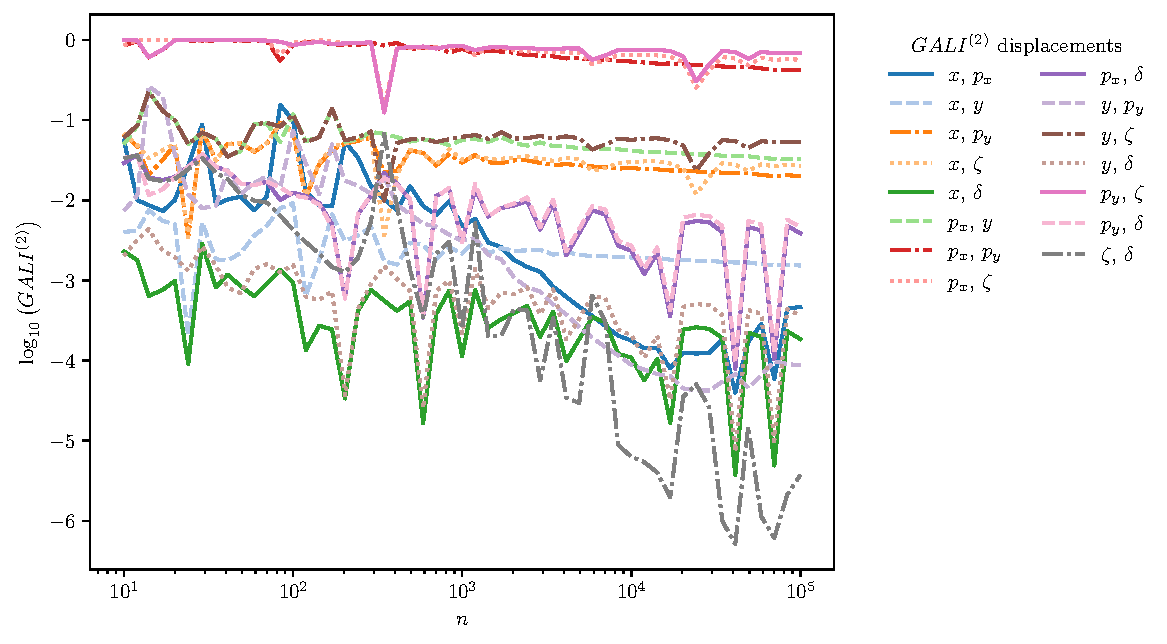
\includegraphics[width=0.8\textwidth]{6_lhc_dynamic_indicators/figs/evolution_gali_2_stable.pdf}
    \caption{Evolution of the mean value of the $GALI^{(2)}$ indicator for different displacement choices. An ensemble of regular initial conditions was considered. The mean value of $GALI^{(2)}$ turns out to remain constant only for the case of displacements that are different from the pairs $(\hat{x},\ \hat{y})$, $(\hat{p}_x,\ \hat{p}_y)$, and $(\hat{\zeta},\ \hat{\delta})$. The cases corresponding to these pairs feature a power law evolution, instead. (HL-LHC lattice used: worst seed, $\zeta_0=$\SI{0.3}{\meter}.)}
    \label{fig:gali2}
\end{figure}

For the indicator $GALI^{(4)}$, the results are shown in Fig.~\ref{fig:gali4}, where we can observe how the mean value of $GALI^{(4)}$ indeed follows a different evolution of the power law depending on the choice of displacement. Moreover, we can observe that all cases also manifest a saturation behaviour for $n>10^4$. To compare the different behaviours, we fit the power law over the interval $10^2\leq n \leq 10^4$, and we report the values of the exponent in Table~\ref{tab:gali4}, along with the corresponding $m$ value. The evolution of $GALI^{(6)}$ is also reported for comparison in both the figure and the table.

We can observe, for the combinations in which the four displacements belong only to two planes, that the exponent of the power law ends up exceeding the value of $2$, which is the maximum expected value of the power law for $k=4$ and $N=3$. For these cases, we reported a negative value of $m$, which does not have a geometrical interpretation. This behaviour as well might be related to the same degeneracy that we have observed for $GALI^{(2)}$, and it will also require further investigation.

Apart from this discrepancy, we can observe how the various displacement choices do yield different values of $m$, which can be interpreted as the number of initial displacements that lie in the tangent space of the regular tori. This is in agreement with the expected behaviour of $GALI^{(4)}$ for regular orbits, and it can be used to inspect the geometry of the regular tori in the phase space, and inspect which vectors lay on the regular tori tangent space.

Finally, $GALI^{(6)}$ shows a power law with exponent $4$, which is higher than all $GALI^{(4)}$ exponents, and implies an $m$ value of $2$. This is in agreement with the expected behaviour of the dynamic indicator.

\begin{figure}
    \centering
    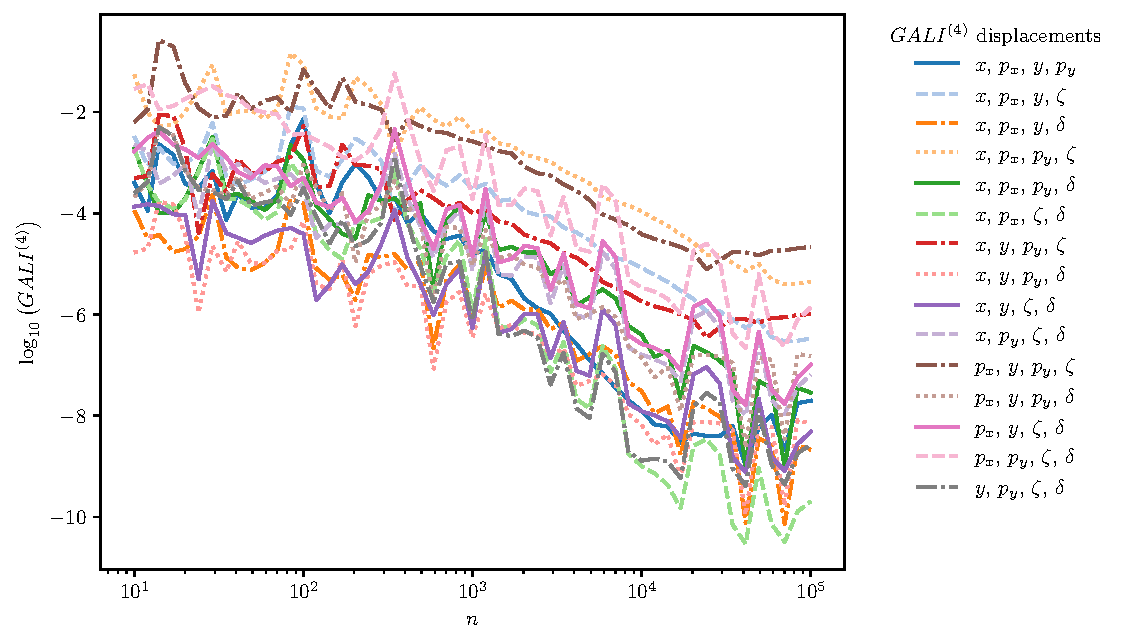
\includegraphics[width=0.8\textwidth]{6_lhc_dynamic_indicators/figs/evolution_gali_4_stable.pdf}
    \caption{Mean value evolution of $GALI^{(4)}$ for different displacement choices. An ensemble of regular initial conditions was considered. The mean value of $GALI^{(4)}$ follows a different power law evolution depending on the displacement choice. (HL-LHC lattice used: worst seed, $\zeta_0=$\SI{0.3}{\meter}.)}
    \label{fig:gali4}
\end{figure}

\begin{table}
    \centering
    % should I space it? nah... let's decide later
    % \setlength{\extrarowheight}{2pt}
    \begin{tabular}{l|cc}
        \toprule
        \makecell{Displacement\\choice} & $2(k-3)-m$ & $m$ \\
        \midrule
        $\hat{x}$, $\hat{p}_x$, $\hat{p}_y$, $\hat{\zeta}$, & $1.25 \pm 0.09$ & $0.75$ \\
        $\hat{x}$, $\hat{p}_x$, $\hat{y}$, $\hat{\zeta}$, & $1.26 \pm 0.09$ & $0.74$ \\
        $\hat{x}$, $\hat{y}$, $\hat{p}_y$, $\hat{\zeta}$, & $1.44 \pm 0.08$ & $0.56$ \\
        $\hat{x}$, $\hat{p}_y$, $\hat{\zeta}$, $\hat{\delta}$, & $1.5 \pm 0.2$ & $0.5$ \\
        $\hat{x}$, $\hat{p}_x$, $\hat{p}_y$, $\hat{\delta}$, & $1.5 \pm 0.2$ & $0.5$ \\
        $\hat{x}$, $\hat{y}$, $\hat{\zeta}$, $\hat{\delta}$, & $1.5 \pm 0.2$ & $0.5$ \\
        $\hat{x}$, $\hat{p}_x$, $\hat{y}$, $\hat{\delta}$, & $1.5 \pm 0.2$ & $0.5$ \\
        $\hat{p}_x$, $\hat{y}$, $\hat{p}_y$, $\hat{\zeta}$, & $1.49 \pm 0.05$ & $0.51$ \\
        $\hat{p}_x$, $\hat{p}_y$, $\hat{\zeta}$, $\hat{\delta}$, & $1.5 \pm 0.2$ & $0.5$ \\
        $\hat{p}_x$, $\hat{y}$, $\hat{\zeta}$, $\hat{\delta}$, & $1.5 \pm 0.2$ & $0.5$ \\
        $\hat{x}$, $\hat{y}$, $\hat{p}_y$, $\hat{\delta}$, & $1.7 \pm 0.1$ & $0.3$ \\
        $\hat{p}_x$, $\hat{y}$, $\hat{p}_y$, $\hat{\delta}$, & $1.7 \pm 0.1$ & $0.3$ \\
        $\hat{y}$, $\hat{p}_y$, $\hat{\zeta}$, $\hat{\delta}$, & $2.5 \pm 0.2$ & $-0.5$ \\
        $\hat{x}$, $\hat{p}_x$, $\hat{\zeta}$, $\hat{\delta}$, & $2.6 \pm 0.2$ & $-0.6$ \\
        $\hat{x}$, $\hat{p}_x$, $\hat{y}$, $\hat{p}_y$, & $2.6 \pm 0.1$ & $-0.6$ \\
        \midrule
        $GALI^{(6)}$ & $4.0 \pm 0.2$ &  2.0 \\   
        \bottomrule     
    \end{tabular}
    \caption{Exponent of the power law and consequent values of $m$ for the different displacement choices for $GALI^{(4)}$. The errors reported correspond to the standard deviation evaluated by the least-squares fit. The exponent of $GALI^{(6)}$ is also reported. (HL-LHC lattice used: worst seed, $\zeta_0=$\SI{0.3}{\meter}.)}
    \label{tab:gali4}
\end{table}

Let us now consider the behaviour of $GALI^{(k)}$ for an ensemble of chaotic initial conditions. We expect both $GALI^{(2)}$ and $GALI^{(4)}$ to exhibit a similar exponential decay, regardless of the displacement choice, with $GALI^{(4)}$ showing a decay rate roughly double that of $GALI^{(2)}$. To check this, we consider the initial conditions that scored a value greater than $10^{-3}$ with $FLI^{WB}(\hat{x})$, evaluated at $n=10^{5}$, and compute the mean value of $GALI^{(2)}$ and $GALI^{(4)}$ scored for each displacement choice.

The results are shown in Fig.~\ref{fig:gali2_4_chaos}. The mean values of $GALI^{(2)}$ and $GALI^{(4)}$ follow an exponential decay in agreement with the expectations. All various displacement choices only exhibit an offset, but all have roughly the same decay rate. The pair $(\hat{\zeta}, \hat{\delta})$, which exhibits a faster decay rate compared to the other displacement choices $GALI^{(2)}$.  

\begin{figure}
    \centering
    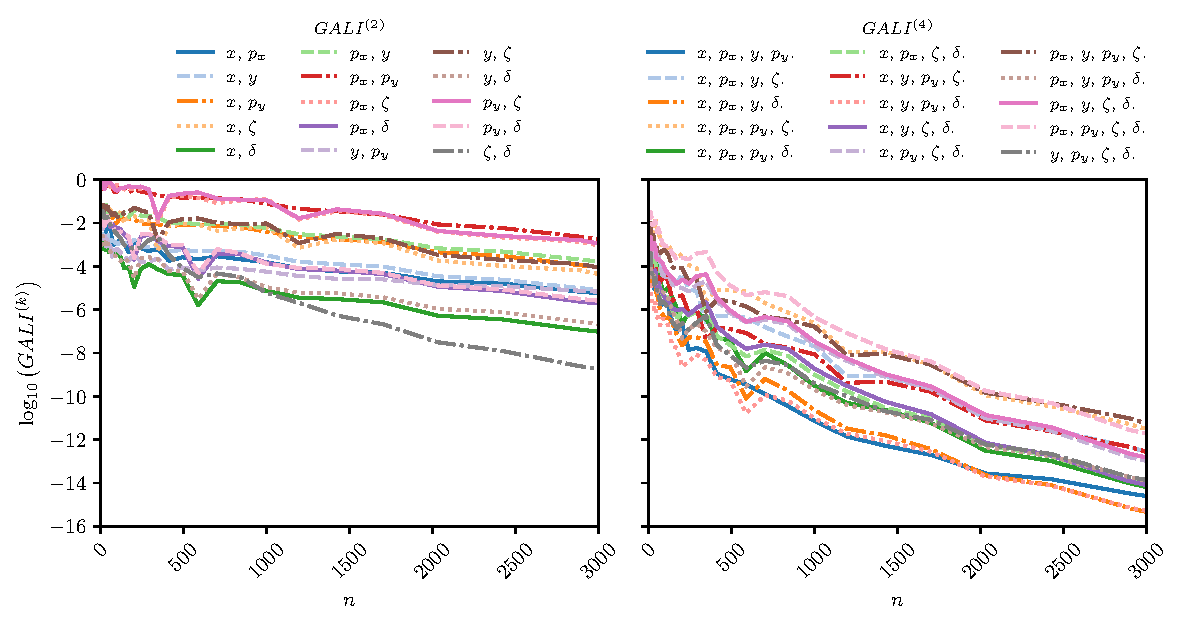
\includegraphics[width=1.0\textwidth]{6_lhc_dynamic_indicators/figs/gali_2_4_chaos.pdf}
    \caption{Mean value evolution of $GALI^{(2)}$ and $GALI^{(4)}$ for different displacement choices. An ensemble of chaotic initial conditions was considered. The mean value of the two $GALI$ indicators both follow an exponential decay, which is in agreement with the expected behaviour for chaotic orbits. $GALI^{(4)}$ shows roughly double the decay rate of $GALI^{(2)}$. The displacement choice $(\hat{\zeta}, \hat{\delta})$ in $GALI^{(2)}$ shows a faster decay rate than the other choices. (HL-LHC lattice used: worst seed, $\zeta_0=$\SI{0.3}{\meter}.)}
    \label{fig:gali2_4_chaos}
\end{figure}


\section{Conclusions and future work}\label{sec:8:conclusions}

In this chapter, we used a set of dynamic indicators to study the beam dynamics generated by a realistic accelerator magnetic lattice. Given the ability of dynamic indicators to provide information on the chaotic character of the dynamics, they can be used to probe the long-term dynamics of charged particles in a circular accelerator, in order to gain insights on the phase-space structures and the scaling laws governing the beam dynamics, which are closely linked to stability and diffusive behaviour.

Five indicators have been considered, namely $FLI/n$, $FLI^{WB}$, $GALI^{(k)}$, $REM$, and $FMA$, based on the experience gained from the study of the dynamics generated by the H\'enon map. The computational aspects and numerical implementation of these indicators have been discussed, and they were then tested on an HL-LHC realistic accelerator lattice, and the information provided by each indicator was discussed, also with emphasis on their features.

We have observed that the $REM$ indicator performs mostly as expected, while the $FMA$ is strongly affected by the tune modulation induced by the longitudinal motion that couples with the transverse one by means of the non-zero chromaticity. In a way, this is comparable to the behaviour observed on the modulated Hénon map in the presence of tune modulation. 

The indicators have also been used to attempt a detailed characterisation of the beam dynamics. We have observed how the Lyapunov time, provided with improved convergence rates by $FLI^{WB}$, can be used to inspect the presence of a Nekhoroshev-like scaling law for the dynamics, and how such value is related to both the lattice realisations and the longitudinal dynamics. This suggests that such a concept can indeed be used to inspect the presence of extended chaotic structures in the phase space, which might be related to long-term Nekhoroshev-like diffusive behaviour. Furthermore, the time evolution of the indicators $GALI^{(k)}$ has been studied for chaotic initial conditions, highlighting some properties, while its use to study the geometry of the regular orbits will be the topic of future studies.
